\documentclass[letterpaper,12pt]{article}

\usepackage{threeparttable}
\usepackage{geometry}
\geometry{letterpaper,tmargin=1in,bmargin=1in,lmargin=1.25in,rmargin=1.25in}
\usepackage[format=hang,font=normalsize,labelfont=bf]{caption}
\usepackage{amsmath}
\usepackage{mathrsfs}
\usepackage{multirow}
\usepackage{array}
\usepackage{delarray}
\usepackage{listings}
\usepackage{amssymb}
\usepackage{amsthm}
\usepackage{lscape}
\usepackage{natbib}
\usepackage{setspace}
\usepackage{float,color}
\usepackage[pdftex]{graphicx}
\usepackage{pdfsync}
\usepackage{verbatim}
\usepackage{placeins}
\usepackage{geometry}
\usepackage{pdflscape}
\synctex=1
\usepackage{hyperref}
\hypersetup{colorlinks,linkcolor=red,urlcolor=blue,citecolor=red}
\usepackage{bm}
\usepackage{setspace}
\doublespacing


\theoremstyle{definition}
\newtheorem{theorem}{Theorem}
\newtheorem{acknowledgement}[theorem]{Acknowledgement}
\newtheorem{algorithm}[theorem]{Algorithm}
\newtheorem{axiom}[theorem]{Axiom}
\newtheorem{case}[theorem]{Case}
\newtheorem{claim}[theorem]{Claim}
\newtheorem{conclusion}[theorem]{Conclusion}
\newtheorem{condition}[theorem]{Condition}
\newtheorem{conjecture}[theorem]{Conjecture}
\newtheorem{corollary}[theorem]{Corollary}
\newtheorem{criterion}[theorem]{Criterion}
\newtheorem{definition}{Definition} % Number definitions on their own
\newtheorem{derivation}{Derivation} % Number derivations on their own
\newtheorem{example}[theorem]{Example}
\newtheorem{exercise}[theorem]{Exercise}
\newtheorem{lemma}[theorem]{Lemma}
\newtheorem{notation}[theorem]{Notation}
\newtheorem{problem}[theorem]{Problem}
\newtheorem{proposition}{Proposition} % Number propositions on their own
\newtheorem{remark}[theorem]{Remark}
\newtheorem{solution}[theorem]{Solution}
\newtheorem{summary}[theorem]{Summary}
\bibliographystyle{aer}
\newcommand\ve{\varepsilon}
\renewcommand\theenumi{\roman{enumi}}
\newcommand\norm[1]{\left\lVert#1\right\rVert}

\begin{document}

\title{581 Project\\Overlapping Generations Model}
\author{Chris Rytting}
\maketitle
	Overlapping generations models have been a prominent tool in economic modeling since 1958, when they were first introduced by Samuelson. They allow for rich heterogeneity between agents, and proffer two primary benefits. Firstly, agents can take on diverse ages, which is an important factor in economic decision-making. Secondly, these models assume that the lives of these agents must ultimately end, a fairly intuitive and sensible assumptions. These models are pivotal in exploring questions concerning policies that have different impacts on an agent depending on his or her age. \\
\indent	In this particular model, we will calculate the trajectories of aggregate labor supply and capital stock over the course of a specified time period $T$. There is one individual born in every period. Let age be indexed by \[s  = \{1,2,\dots,S\}\] through whatever $S$ the user specifies. Each individual has the following budget constraint:
    \[c_{s,t} + b_{s+1,t+1} = w_t n_{s,t} + (1 + r_t)b_{s,t}\]
where $c$ is consumption, $b$ is savings, $w$ represents wages, $r$ represents the interest rate, and $n$ represents labor. Let the interest rate and wages be expressed as the marginal product of capital and the marginal product of labor, respectively. If we have that firms use their capital $K_t$ and labor $L_t$ to produce output $Y_t$ at every period $t$ according to a Cobb-Douglas production function
\[ Y_t = AK_t^\alpha L_t^{1-\alpha} \quad \alpha \in (0,1), \quad A > 0\]
then we have that the first order conditions yield
\[r_t = \alpha A \left( \frac{L_t}{K_t} \right)^{1-\alpha} - \delta\]
where $\delta$ is the depreciation rate and
\[w_t = (1-\alpha) A \left( \frac{K_t}{L_t} \right)^{\alpha} \]

We will assume that individuals are born with no savings and they do not save anything in the last period of their lives, or more precisely that
\[b_{1,t} = 0 \quad b_{S,t} = 0\quad  \forall t\]
We impose the condition that individuals cannot have negative consumption, or that 
\[c_{s,t} > 0 \quad  \forall t\]
However, individuals can borrow. Now, we will define the utility function $u(c_{s,t})$ as follows:
\[ u(c_{s,t},n_{s,t}) = \frac{c_{s,t}^{1-\gamma} - 1}{1 - \gamma} + \frac{(1-n_{s,t})^{1+\theta}}{1+\theta}\]
with the parameter $\gamma > 1$ being a coefficient representing relative risk aversion and the parameter $\theta \geq 0$ being a coefficient inversely proportional to the Frisch elasticity of labor supply. This is an appropriate function to choose as, if an individual consumes nothing, the limit of the function nears negative infinity, penalizing an individual's behavior which would, in real life, lead to death. The negative part of the utility function represents the disutility of working that an individual experiences.\\
\indent Individuals choose, over the course of their lifetimes, individual consumption $\{c_{s,t+s-1}\}_{s=1}^S$, labor supply $\{n_{s,t+s-1}\}_{s=1}^S$, and savings $\{b_{s+1,t+s}\}_{s=1}^{S-1}$ to maximize lifetime utility. We do have a budget constraint, however, and so by simply substituting our budget constraint into the maximization problem, we can naturally constrain it and get the desired result. So where we have the problem
\[ \text{max}_{\{c_{s,t+s-1},n_{s,t+s-1}\}_{s=1}^S,\{b_{s+1,t+s}\}_{s=1}^{S-1}} ~ ~ ~u(c_{1,t}n_{1,t}) + \beta u(c_{2,t+1}n_{2,t+1}) + \cdots + \beta^{S-1} u(c_{S,t+S - 1}n_{S,t+ S -1})\]
subject to
\[ c_{1,t} = w_tn_{1,t} - b_{2,t+1} \]
\[ c_{2,t+1} = w_{t+1}n_{2,t+1} + (1+r_{t+1})b_{2,t+1} - b_{3,t+2} \]
\[\vdots\]
\[ c_{S,t+S-2} = w_{t+S-2}n_{S-1,t+ S-2} + (1+r_{t+S-1})b_{S-1,t+S-2} - b_{S,t+S} \]
\[ c_{S,t+S-1} = w_{t+S-1}n_{S,t+ S-1} + (1+r_{t+S-1})b_{S,t+S-1}\]
since labor and savings are implicit in consumption, we only have $2S-1$ decisions to make instead of $3S - 1$, and we will only take first order conditions for savings and capital. This differentiation yields the following first order conditions: $S$ dynamic Euler equations for labor
\[w_tu_1(c_{s,t}n_{s,t}) = -u_2(c_{s,t} n_{s,t}) \quad \forall t,s\]
and $S-1$ dynamic Euler equations for savings
\[u_1(c_{s,t}, n_{s,t}) = \beta (1 + r_{t+1}) u_1 (c_{s+1, t+1}, n_{s+1, t+1})\quad  \forall t,s \]
where 
\[u_1(c_{s,t}, n_{s,t}) = c_{s,t}^{-\gamma} \]
\[u_2(c_{s,t}, n_{s,t}) = (1 - n_{s,t})^{-\theta} \]
Now, these maximizations depend on the values of the interest rate over time $\{r_v\}_{v=0}^{t+2}$, and wages over time $\{w_v\}_{v=0}^{t+2}$, and if households know what prices will be, then our system of equations is perfectly identified and we can solve this system of Euler equations.\\
\indent In order for markets to clear, we need the following three conditions to hold:
\[L_t = \sum^{S}_{s=1} n_{s,t} \]
\[K_t = \sum^{S}_{s=2} b_{s,t} \]
\[Y_t = C_t + K_{t+1} - (1 - \delta) K_t\]
Now, we can characterize equilibrium by the fulfillment of three conditions:
\begin{enumerate}
\item Firms optimizing according to wage and interest specifications given previously.
\item Households maximizing lifetime utility.
\item Markets clearing according to specifications given previously.
\end{enumerate}
Given this information, we can first find a steady state by making an educated guess as to what the eventual distribution of savings and labor will be for individuals in this economy. Using this guess, we use an ``fsolve'' method in python to solve the system of equations that yields a distribution of capital stocks and labor supplies in the steady state. This distribution tells us just what each individual will tend towards deciding in terms of labor and savings during each period of their lives.
\\
\indent Once we have the steady state distribution, we can discover something else about the economy: given a shock to the steady state distribution of savings and labor, what will the trajectory look like returning to the steady state. Essentially, we can assume that, for whatever reason, people are saving twice as much and working half as much as they would in the long run. This will cause the aggregate savings and labor to be different, and this in turn will cause the wage and interest rate to change. We know, however, that all of these variables will settle down to the steady state values over the course of time. We can make a conjecture, then, as to what the wage rate, interest rate, savings and labor will be over the course of many years, and by plugging in this guess to the Euler equations, we will get a new aggregate capital stock and a new aggregate labor supply, resulting in new wage and interest rates, which we will use as updated guesses and repeat the process. \\
\indent Now, a quick digression: There are various ways to measure the distance between two curves on a graph. There is a class of these distance measures called norms. A ``1-norm'' takes the absolute value of the difference of the graphs at every point it is measured. The ``infinity norm'' measures the supremum of these differences. The norm we will use to measure distance is the standard Euclidean norm, where we square the differences, sum them, and then take the square root to find our distance measure.\\
\indent Returning to the discussion of our method of updating guesses, any given guess should be closer to the guess it yields than to the guess it came from. That is to say, the norm of each two guesses should progressively get smaller until it is almost zero. This process is called Time Path Iteration, and we use it to find the trajectories of aggregate capital stock and labor supply over time. 

\subsection*{Results}
The results for a ten-period model are as follows:\\\\
Capital Steady States:
\[ 
\begin{bmatrix}
0.03339802\\
0.06762161\\
0.10193072\\
0.1350282\\
0.16469442\\
0.18718515\\
  0.19623941\\
  0.18144474\\
  0.12554422
\end{bmatrix}
\]
We can see here that the trajectory of capital rises over the first part of life and then declines. This is consistent with our economic intuition as individuals save most when they are earning the most, right around the middle of their lives. \\\\

Labor Steady States:
\[
\begin{bmatrix}
 0.68710735\\
 0.66792835\\
 0.64757376\\
 0.62597152\\
 0.60304516\\
 0.5787135\\
  0.55289042\\
  0.52548449\\
  0.49639869\\
  0.46553006
\end{bmatrix}
\]
Individuals seem to work less and less as time goes on. This is also in line with our economic intuition, as wealth accumulates over the lifetime and individuals have the liberty to decrease their workload over time.

\indent Now, if we shock the steady state distributions by $-10$ percent, then we get the following time paths:\\\\\\
\\\\
\\\\\\\\\\




\begin{figure}[h] 
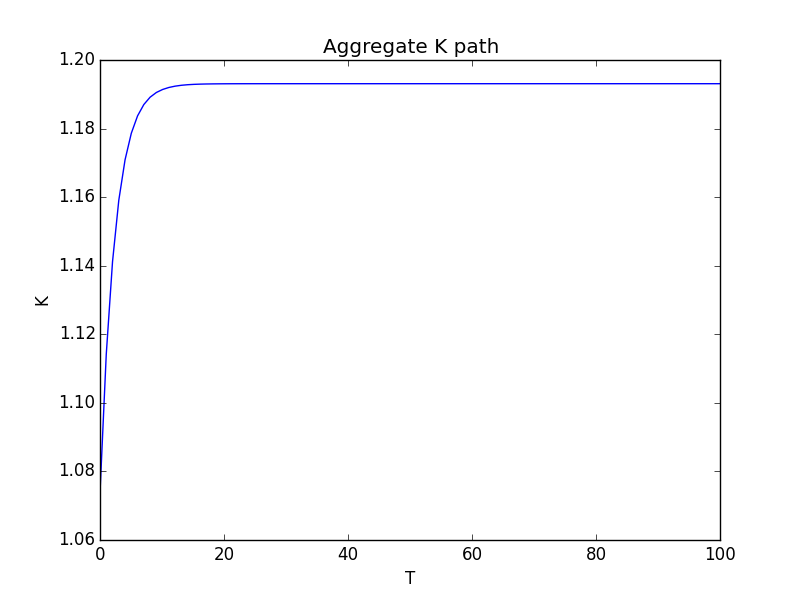
\includegraphics[scale = .5]{10periodK.png}
\centering 
\caption{10 period capital trajectory}
\end{figure}
\begin{figure}[h] 
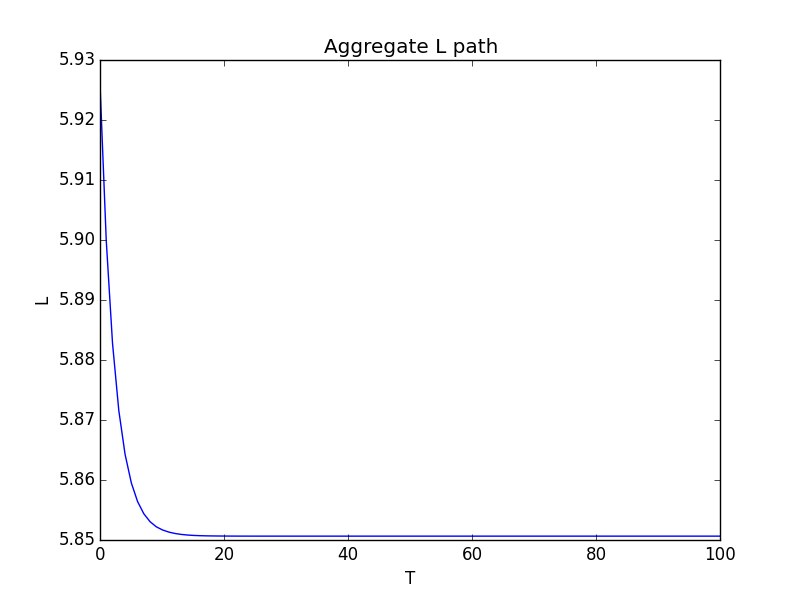
\includegraphics[scale = .5]{10periodL.png}
\centering 
\caption{10 period labor trajectory}
\end{figure}

We can see in figures 1 and 2 that the capital stock and labor supply reach their steady-state values in $10-15$ periods. This suggests that the capital stock in period $0$ gradually increases until it reaches the steady state indicated at the beginning of the results section. The labor stock decreases in like fashion, with individuals working more initially due to the adverse conditions of the economy.\\\\
\\\\
\\\\\\\\\\\\




\begin{figure}[h] 
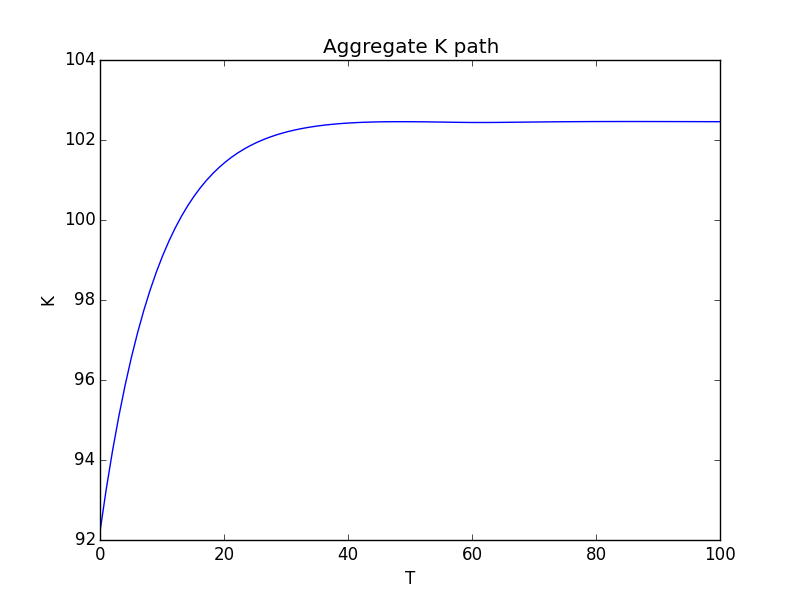
\includegraphics[scale = .5]{80periodK.png}
\centering 
\caption{80 period capital trajectory}
\end{figure}
\begin{figure}[h] 
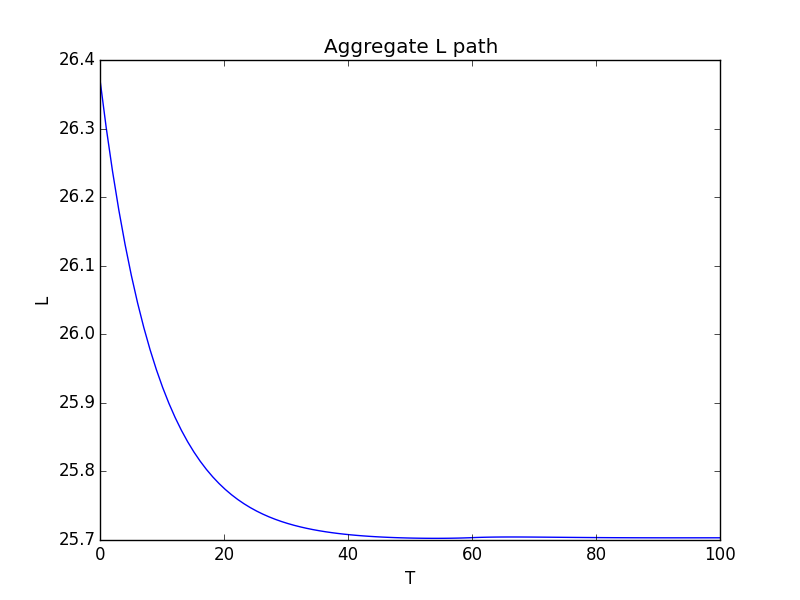
\includegraphics[scale = .5]{80periodL.png}
\centering 
\caption{80 period labor trajectory}
\end{figure}


If we have more agents, however, who live for longer, say $S = 80$, then we get a slightly different result, as seen below. It takes a longer time for the labor and capital stocks to adjust to the steady states. However, the same results, of capital increasing over time and labor decreasing over time, hold just as in the case where $S = 10$ (Omitted are the steady state vectors, as there are $159$ values, quite a lengthy list). The trajectories are as follows in figures 3 and 4:




\end{document}
